\subsection {Session 12, Exercise 9}
\label{13f9}

\lineparagraph {Exercise}

Hash function $h(x) = x~ \pmod{M}$ is used in open addressing hash to insert keys $4,5,14,15,16,26,3$ in this
order into an initially empty table of size $M = 11$. Show the resulting table if

\begin{enumerate}[a)]
    \item linear probe is used
    \item quadratic probe is used
    \item double hashing is used with second hash function $h'(x) = 7x~ \pmod{(M-1)}$ is used
\end{enumerate}

for collision resolution. How many collisions occure in each case?


\lineparagraph {Solution}

All types of open hashings try in the original $h(x)$ position first. When a collision happens, they try the following offsets:

\begin{itemize}
    \item Linear probing starts to the left, and tries the offsets $-1, -2, -3, \dots$ etc.
    \item Quadratic probing starts to the \textbf{right} (!), and tries the offsets $+1, -1, +4, -4,  +9, -9 \dots$ etc (square numbers).
    \item Double hasing uses a secondary hash function, h'(x) and tries the offsets $-1\cdot{}h'(x), -2\cdot{}h'(x), -3\cdot{}h'(x), \dots$ etc.
\end{itemize}

Whenever you run out at the end of the array, you come back at the other. (Or, you can imagine the indexing having a mod tablesize applied to it.)

The offsets are not cumulative, all of them are applied to the original h(x).

\begin{center}
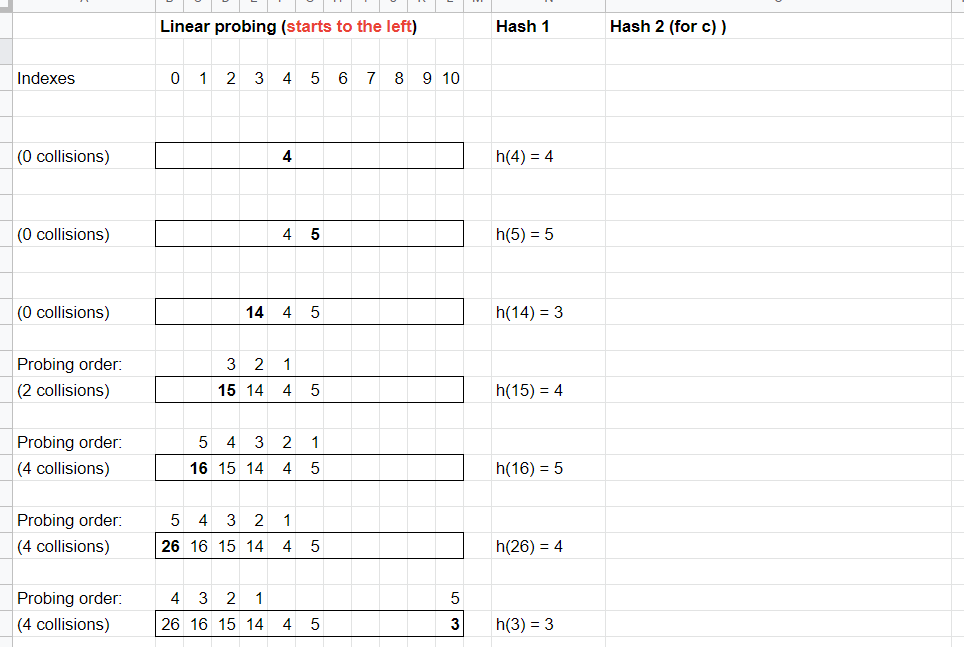
\includegraphics[width=\linewidth]{./12/09/linear.png}
\end{center}
\separate
\begin{center}
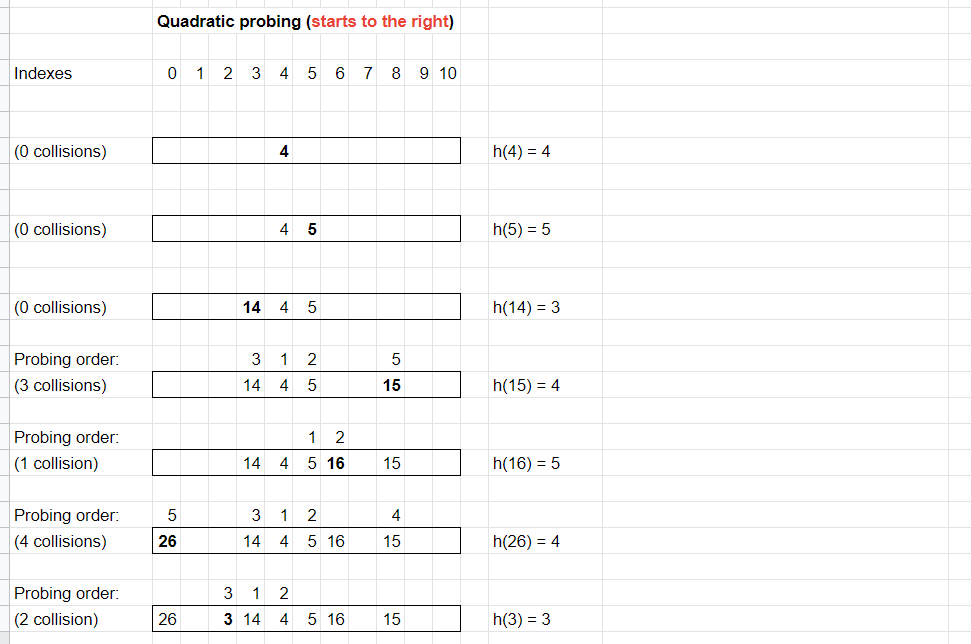
\includegraphics[width=\linewidth]{./12/09/quadratic.png}
\end{center}
\separate
\begin{center}
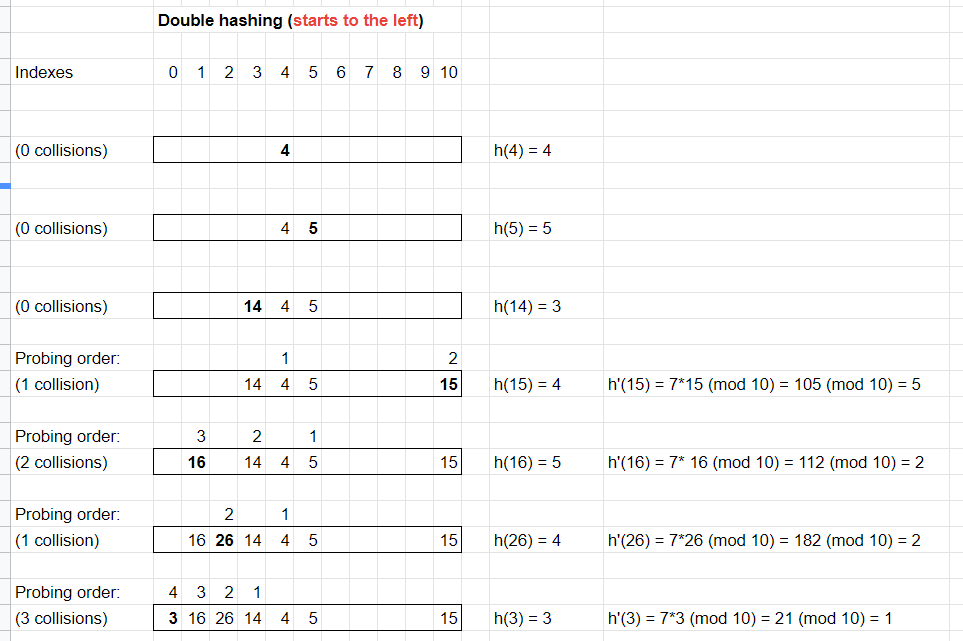
\includegraphics[width=\linewidth]{./12/09/double.png}
\end{center}